\documentclass[twocolumn]{article}
\usepackage{datetime}
\usepackage{hyperref}
\usepackage{listings}
\usepackage{color}
\usepackage{graphicx}

\begin{document}

% Source code highlighting
\definecolor{javared}{rgb}{0.6,0,0} % for strings
\definecolor{javagreen}{rgb}{0.25,0.5,0.35} % comments
\definecolor{javapurple}{rgb}{0.5,0,0.35} % keywords
\definecolor{javadocblue}{rgb}{0.25,0.35,0.75} % javadoc
\lstset{language=Java,
	basicstyle=\ttfamily\tiny,
	keywordstyle=\color{javapurple}\bfseries,
	stringstyle=\color{javared},
	commentstyle=\color{javagreen},
	morecomment=[s][\color{javadocblue}]{/**}{*/},
	numbers=none,
	stepnumber=2,
	numbersep=10pt,
	tabsize=2,
	showspaces=false,
showstringspaces=false,
framesep=0pt}

% Title
\pagenumbering{gobble}
\begin{titlepage}


\vspace*{15em}


\centering

{\LARGE
Department of Electrical \& Computer Engineering \\
Final Year Research Project 2015, Interim Report}

\hspace{2em}

% notes on latex tables use "&" as colum sperator
\begin{table*}[h]
\centering
\begin{tabular}{ll}
Project Title: & Preventing plagiarism during practical tests \\
Project Number: & 11 \\
Supervisor Name: & Dr Nasser Giacaman \\
Second Examiner Name: & Avinash Malik \\
Your Name: & Kurt McAlpine \\
Your UID: & 2004750 \\
Partner Name: & Conor Simmonds \\
Date submitted: & 11\textsuperscript{th} May 2015 \\

\end{tabular}
\end{table*}
\begin{table}


\end{table}
\pagebreak

\vspace*{25em}

{\Large Declaration of Originality}

\hspace{5em}

This report is my own unaided work and was not copied from 
nor written in collaboration with any other person.

Name: Kurt McAlpine


\end{titlepage}



\pagenumbering{arabic}

\begin{abstract}

Software engineering courses today have impractical test environments. They are
performed using pen and paper, without access to a computer, compiler, IDE or
the internet. Active Test Programmer gives the students the opportunity to be
tested in a practical manner and gives the teacher confidence that plagiarism
will be caught. Practical tests will give students a more realistic assessment
of their abilities in the real world. Practical tests also give industry
recruiters more confidence that students that graduate from such programmes have
good practical skills. 

\end{abstract}

\section{Introduction}
In the world today, programming and programs are prevalent and abundant in our
every day lives. Therefore it is an important skill. It's
widely accepted that programming is a difficult skill to learn
\cite{jenkins2002difficulty, robins2003learning}. There is a need to innovate
and devise solutions to help students be more effective in class.
When students struggle in class with tests and assignments, it can lead to
plagiarism or even dropping out\cite{bennedsen2007failure}. Currently in many
institutions, software engineering courses test their students on their
knowledge and skill in a way that is artificial to real world programming.
For example, tests are done with pen and paper and without access to computers with
IDE`s, compilers or the internet. Therefore, in this project we want to construct a
way to give software engineering students robust testing environments that allow
students to have a more realistic set of tools during the test. However, whilst
giving students these tools we would also like to give the teaching staff
confidence that plagiarism can be detected automatically without tedious manual
inspection of student submissions as well as detecting plagiarised work that the
student has attempted to conceal.
% TODO overview of report

\section{Background}
Eclipse is an IDE (Integrated Development Environment) that is written in Java.
It can be used to develop in a variety of programming languages. It also has
a plugin architecture which allows other developers to extend its functionality
without changing its core implementation.

There are several plagiarism detection tools available for institutions to use.
Two of which are MOSS\cite{schleimer2003winnowing} and
JPlag\cite{lutz2000jplag}. Both these systems are utilised on submissions from
students to help identify any similarities between the students' work. If the student
submissions are too similar, these tools will detect that and warn the lecturer
that plagiarism is the likely cause of this similarity.

A tool called ACP (Active Classroom Programmer)\cite{giacaman2015active} is used
at the University of Auckland in SOFTENG 701 and 751. ACP is an eclipse
plugin that allows the lecturer to create eclipse workspaces and upload
snapshots of the current state to a web server. For example during a lecture a
task can be completed in parts and once each part is complete a snapshot of the
code can be uploaded. The students, during the lecture can download these
snapshots using the ACP eclipse plugin, onto their laptops and make
modifications and experiment with the workspace, they can also attempt to
complete the next part before the lecturer has completed it. Often there are
short breaks during the lecture that allow students to attempt the tasks.

Active Test Programmer (ATP) is an extension to ACP which allows the lecturer to
setup a programming test. The programming test can be distributed to students
before the test starts. The test is encrypted so a secret code is needed to
decrypt the tests. When a secret code is distributed to the students they may
type it in and begin the test. After a predetermined amount of time the the test
is over and the students must submit their code through the eclipse plugin.

\section{Active Test Programmer}
For my project, we are going to extend ATP to give lecturers confidence that
plagiarism that has occurred during the test can be detected automatically. The
way this will be done is the history of the student completing the test will be
recorded and when the test is submitted the history will go with it. This
history gives us much richer insight into the characteristics of the students
work. Analysis of the history of the students submission will allow for more
robust detection of potential plagiarism.

\subsection{Features} \label{sec:Features}
Create tests: The lecturer will be able to create a programming test in their
IDE and upload it. Once the test is uploaded the lecturer will be given a secret
code that can be used to begin the test.

Download tests: Students will be able to download tests from within their IDE,
they may not begin the test until they have entered the secret code to decrypt
the test. This allows all the students to download and be ready for the test, so
that everyone may begin at the same time, and no students will feel
disadvantaged because it took them longer to download the test, or if WiFi is
unavailable the test may be distributed on a USB flash drive.

Upload completed test: Students may upload their completed test through their
IDE. If WiFi is unavailable they may export their completed test to an archived
file and copy it to a flash drive to give to the lecturer. The archived
completed test will contain information about when it was exported so that we
can be sure they completed the test in the given time.

Implementation history: The completed test that the student uploads, will
contain a complete history in snapshots over time of how the test was
implemented. This gives a rich insight into potential plagiarism in the history
of the code.

Viewing reports: Reports can be generated that contain analyses of student
tests. In the analyses it will contain a score of how likely it was that the
students submission contains plagiarised work. The history also gives us the
opportunity to go beyond just checking for plagiarism.

\section{Technologies Considered}
For this project the client application will be implemented using the Eclipse
plugin framework. There are other IDE's that could potentially be used because
it also have a plugin architecture for example IntelliJ but Eclipse was chosen
because ACP is already implemented for Eclipse and it's going to be extended to
contain the features outlined in \nameref{sec:Features}.

For recording the history of the changes to files in the students test, libgit2
will be used. libgit2 can be used to store the history of a file in a series of
commits. The reason libgit2 will be used is that is has a permissive license so
it can be integrated into this project without license concerns. Implementing a
system of storing changes to a file isn't feasible for a small project like this
so libgit2 is a good fit.

\section{Implementation}

I have implemented several components that make up the software solution for my
project. First is the Eclipse Plugin which is an end user oriented plugin
available for students to install onto their machines. Code Report Tool is a
command line application used for the analysis of individual test submissions.
Finally Code Analysis Tool is used in conjunction with Code Report Tool to
aggregate information retrieved from multiple student test submissions.

\subsection{Eclipse Plugin}

\begin{figure}[h!]
\centering
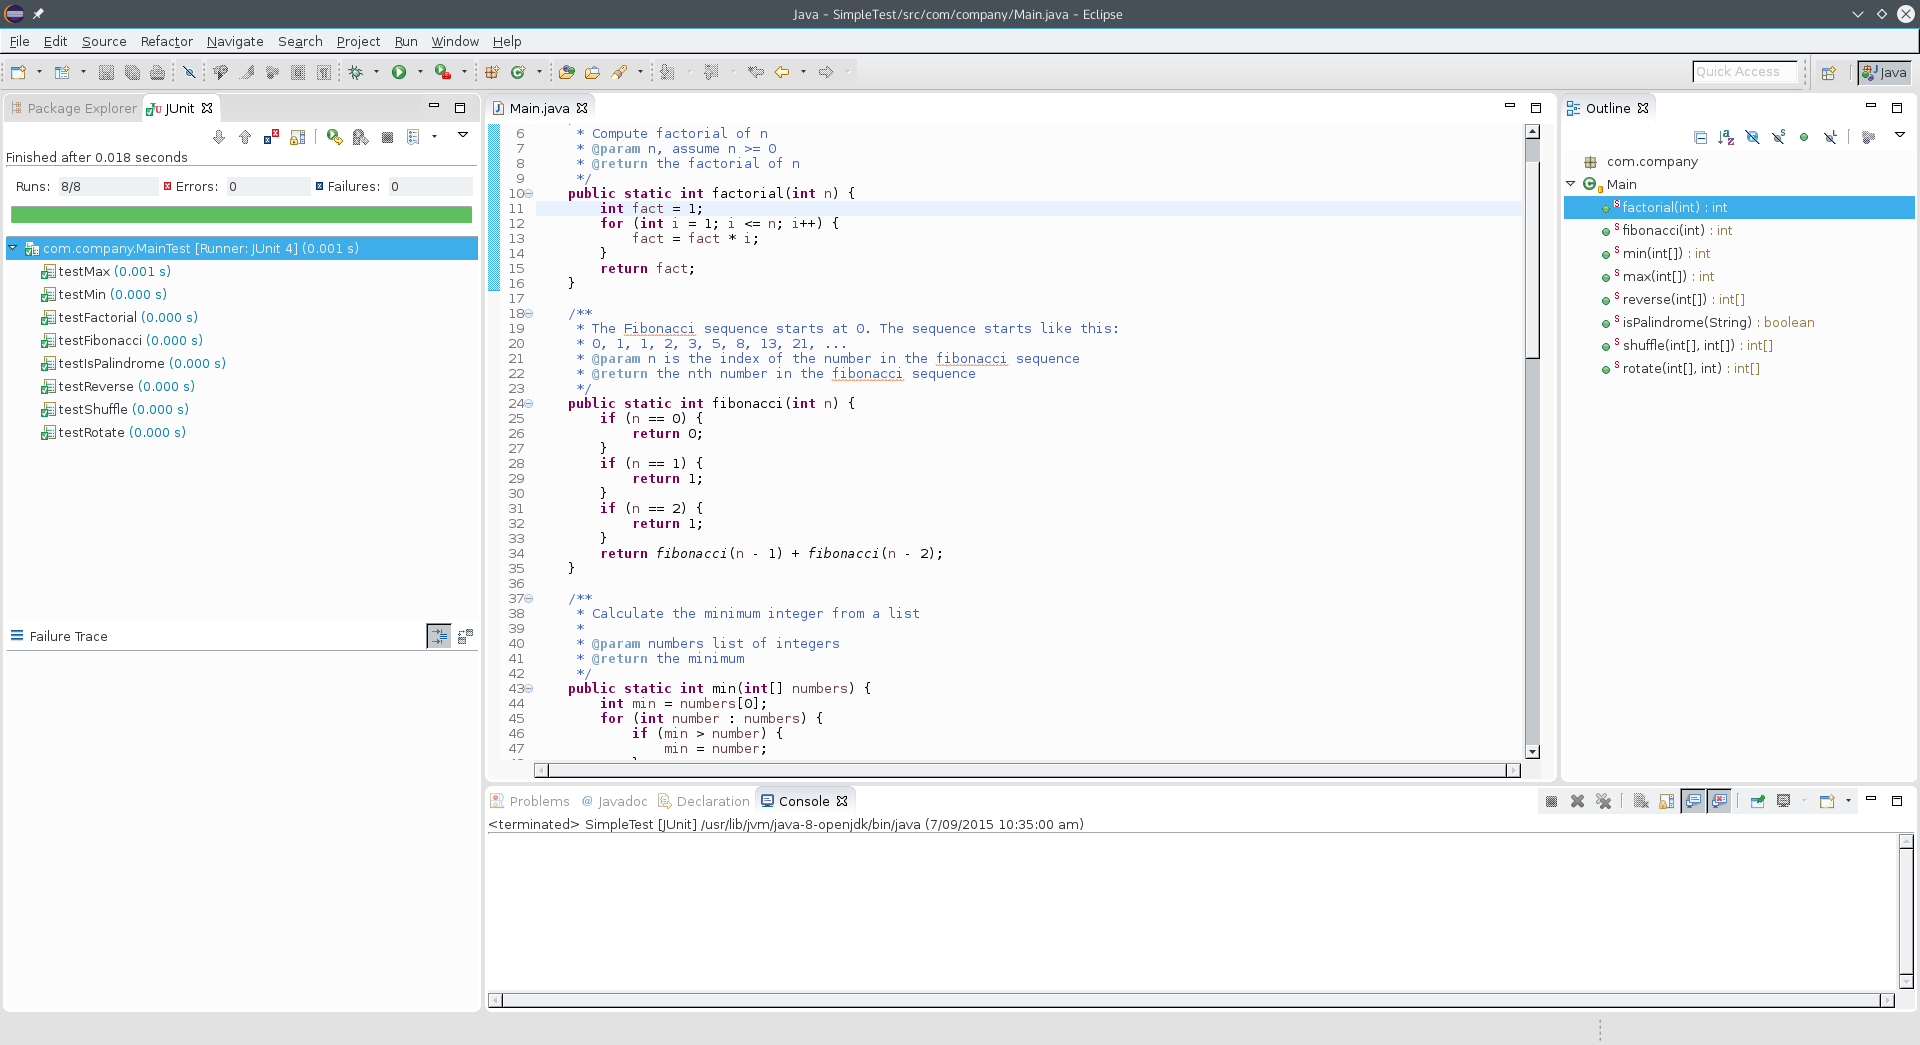
\includegraphics[width=\linewidth]{figures/eclipse}
\caption{Screenshot of a test in progress}
\end{figure}

\subsection{Code Report Tool}
\subsection{Code Analysis Tool}

An example of the series of snapshots that can be retrieved from a repository
are shown below. The following are snapshots from a test that I completed, all
the snapshots are able to be parsed by the Java compiler.
\begin{lstlisting}[frame=single]
public static int max(int[] numbers) {
	return 	0;
}
\end{lstlisting}
\begin{lstlisting}[frame=single]
public static int max(int[] numbers) {
	int max = numbers[0];
	return 	0;
}
\end{lstlisting}
\begin{lstlisting}[frame=single]
public static int max(int[] numbers) {
	int max = numbers[0];
	for (int i = 0; i < numbers.length; i++) {
	}
	return 	0;
}
\end{lstlisting}
\begin{lstlisting}[frame=single]
public static int max(int[] numbers) {
	int max = numbers[0];
	for (int i = 0; i < numbers.length; i++) {
		if (max < numbers[i]) {
		}
	}
	return 	0;
}
\end{lstlisting}
\begin{lstlisting}[frame=single]
public static int max(int[] numbers) {
	int max = numbers[0];
	for (int i = 0; i < numbers.length; i++) {
		if (max < numbers[i]) {
			max = numbers[i];
		}
	}
	return 	0;
}
\end{lstlisting}
\begin{lstlisting}[frame=single]
public static int max(int[] numbers) {
	int max = numbers[0];
	for (int i = 0; i < numbers.length; i++) {
		if (max < numbers[i]) {
			max = numbers[i];
		}
	}
	return 	max;
}
\end{lstlisting}

\section{Evaluation}
To evaluate the effectiveness of the tool, mock tests will be performed with
volunteers to gather some test data. Some of the volunteers will be asked to
copy one another and conceal it. These submissions will be used to evaluated the
accuracy of plagiarism detection. It will also be a good opportunity to get user
feedback and find out about potential bugs and problems before the tool is used
in a more realistic setting.

\section{Conclusions}
Many student tests today to not assess students in a practical manner. The
reason I think that pen and paper tests are popular is because lecturers are
concerned that practical tests will give students an easy opportunity to
plagiarise work.  The goal of Active Test Programmer (ATP) is to remove doubt
from lecturers that plagiarism will be caught. ATP gives confidence to lecturers
that attempts at concealing plagiarism will be found in the history of the
students work. More over plagiarism detection is just one of the benefits of
looking into the history of the code. In fact a more general analysis could give
us information about where the student may have been struggling during the test
by looking at how long it took a student took to implement a particular method
or class. This information could be used to guide the lecturer on which topics
to focus on in class and therefore give students a more effective learning
experience.

\bibliographystyle{IEEEtran}
\bibliography{references}

\end{document}
